\documentclass[]{article}
\usepackage{lmodern}
\usepackage{setspace}
\setstretch{1.5}
\usepackage{amssymb,amsmath}
\usepackage{ifxetex,ifluatex}
\usepackage{fixltx2e} % provides \textsubscript
\ifnum 0\ifxetex 1\fi\ifluatex 1\fi=0 % if pdftex
  \usepackage[T1]{fontenc}
  \usepackage[utf8]{inputenc}
\else % if luatex or xelatex
  \ifxetex
    \usepackage{mathspec}
  \else
    \usepackage{fontspec}
  \fi
  \defaultfontfeatures{Ligatures=TeX,Scale=MatchLowercase}
\fi
% use upquote if available, for straight quotes in verbatim environments
\IfFileExists{upquote.sty}{\usepackage{upquote}}{}
% use microtype if available
\IfFileExists{microtype.sty}{%
\usepackage[]{microtype}
\UseMicrotypeSet[protrusion]{basicmath} % disable protrusion for tt fonts
}{}
\PassOptionsToPackage{hyphens}{url} % url is loaded by hyperref
\usepackage[unicode=true]{hyperref}
\hypersetup{
            pdfborder={0 0 0},
            breaklinks=true}
\urlstyle{same}  % don't use monospace font for urls
\usepackage[left=3cm, right=3cm, top=2cm, bottom=2.5cm]{geometry}
\usepackage{longtable,booktabs}
% Fix footnotes in tables (requires footnote package)
\IfFileExists{footnote.sty}{\usepackage{footnote}\makesavenoteenv{long table}}{}
\usepackage{graphicx,grffile}
\makeatletter
\def\maxwidth{\ifdim\Gin@nat@width>\linewidth\linewidth\else\Gin@nat@width\fi}
\def\maxheight{\ifdim\Gin@nat@height>\textheight\textheight\else\Gin@nat@height\fi}
\makeatother
% Scale images if necessary, so that they will not overflow the page
% margins by default, and it is still possible to overwrite the defaults
% using explicit options in \includegraphics[width, height, ...]{}
\setkeys{Gin}{width=\maxwidth,height=\maxheight,keepaspectratio}
\IfFileExists{parskip.sty}{%
\usepackage{parskip}
}{% else
\setlength{\parindent}{0pt}
\setlength{\parskip}{6pt plus 2pt minus 1pt}
}
\setlength{\emergencystretch}{3em}  % prevent overfull lines
\providecommand{\tightlist}{%
  \setlength{\itemsep}{0pt}\setlength{\parskip}{0pt}}
\setcounter{secnumdepth}{0}
% Redefines (sub)paragraphs to behave more like sections
\ifx\paragraph\undefined\else
\let\oldparagraph\paragraph
\renewcommand{\paragraph}[1]{\oldparagraph{#1}\mbox{}}
\fi
\ifx\subparagraph\undefined\else
\let\oldsubparagraph\subparagraph
\renewcommand{\subparagraph}[1]{\oldsubparagraph{#1}\mbox{}}
\fi

% set default figure placement to htbp
\makeatletter
\def\fps@figure{htbp}
\makeatother


\author{}
\date{\vspace{-2.5em}}

\begin{document}

\selectlanguage{spanish}

\tableofcontents

\section{Introducción y marco del
informe}\label{introducciuxf3n-y-marco-del-informe}

En el presente informe se muestra el resultado de la valoración
económica de diversas alternativas selvícolas planteadas para masas de
Pinus pinaster en el marco del proyecto del Grupo Operativo SIGCA para
madera de calidad de esta especie.

\subsection{Objetivos}\label{objetivos}

\begin{center}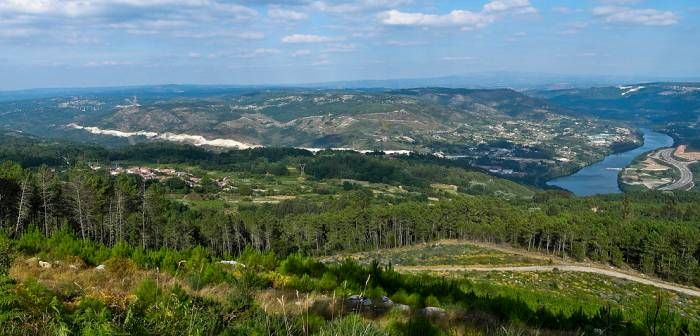
\includegraphics[width=750px]{./imagenes/pinares_92f650725ebb0a7b902f15aebd658059} \end{center}

El objetivo principal de este trabajo es describir la rentabilidad de
cuatro alternatívas selvícolas, cuyas características se presentan a
continuación:

\begin{enumerate}
\def\labelenumi{\arabic{enumi}.}
\tightlist
\item
  M2-Estándar habitual
\end{enumerate}

\begin{itemize}
\tightlist
\item
  Objetivo de gestión: Troncos de 1 a 1,2 m\textsuperscript{3}
\item
  Preparación del terreno: Laboreo en líneas. Fertilización.
\item
  Composición del rodal: Monoespecífica
\item
  Estructura del rodal: Masa regular
\item
  Material genético: Plantas genéticamente mejoradas.
\item
  Tipo de regeneración: Plantación 1250 pies/ha
\item
  Clareo y control de la competencia: Desbroce completo a los 5 años y
  siempre que haya una intervención (4-5 veces con las claras)
\item
  Claras/Podas: 3 claras. Sin podas.
\item
  Aprovechamiento: 40 años; 300 pies/ha
\end{itemize}

\begin{enumerate}
\def\labelenumi{\arabic{enumi}.}
\setcounter{enumi}{1}
\tightlist
\item
  M4-Turno corto con subsídios
\end{enumerate}

\begin{itemize}
\tightlist
\item
  Objetivo de gestión: Troncos pequeños de 0,3 a 0,4
  m\textsuperscript{3}
\item
  Preparación del terreno: Laboreo completo. Fertilización.
\item
  Composición del rodal: Monoespecífica
\item
  Estructura del rodal: Masa regular
\item
  Material genético: Plantas genéticamente mejoradas
\item
  Tipo de regeneración: 1250 pies/ha
\item
  Clareo y control de la competencia: Desbroce completo a los 5 años.
\item
  Claras/Podas: 1 clara. Sin podas.
\item
  Aprovechamiento: 25 años; 700 pies/ha o errática (Galicia)
\end{itemize}

\begin{enumerate}
\def\labelenumi{\arabic{enumi}.}
\setcounter{enumi}{2}
\tightlist
\item
  M8- Sin gestión
\end{enumerate}

\begin{itemize}
\tightlist
\item
  Objetivo de gestión: Sin objetivos productivos
\item
  Preparación del terreno: No
\item
  Composición del rodal: Mixta
\item
  Estructura del rodal: Masa irregular
\item
  Material genético: No.
\item
  Tipo de regeneración: Regeneración natural.
\item
  Clareo y control de la competencia: No
\item
  Claras/Podas: No
\item
  Aprovechamiento: Errático.
\end{itemize}

\begin{enumerate}
\def\labelenumi{\arabic{enumi}.}
\setcounter{enumi}{3}
\tightlist
\item
  MG2-Madera para trituración, sierra y chapa
\end{enumerate}

\begin{itemize}
\item
  Objetivo de gestión: Optimizar la producción económica del monte
  400-500 pies de calidad para madera sólida en la corta final
\item
  Preparación del terreno: Ahoyado mecanizado o subsolado lineal en
  máxima pendiente levantando el subsolador en la linea para evitar
  surcos de escorrentía. Ejecución en tiempo seco, dos meses de
  antelación a la plantación. Raspas picadas de 40x40x20 cm
\item
  Composición del rodal: Monoespecífico
\item
  Estructura del rodal: Masa regular
\item
  Material genético: Preferiblemente mejorado o rodal selecto de origen
  la región de procedencia en que se incluya el monte a repoblar y
  excepcionalmente de otras regiones de procedencias si tiene algún
  nivel de mejora.
\item
  Tipo de regeneración: Plantación a raíz desnuda a savia parada
  (finales de octubre a marzo) y con envase hasta mayo si hay tempero.
  Plantación con barra para asegurarse la colocación de la planta recta.
  Fertilizado NPK bajo en nitrógeno y liberación gradual. También se
  plantea la opción de regeneración natural.
\item
  Clareo y control de la competencia: 8-10 años. dejar 1000-1200 pies/ha
  por lo bajo (sobre árboles dominados y con defectos), o si es
  regenerado natural a 2-5 años clareo-desbroce sistemático por fajas y
  selectivo dentro de la faja que queda hasta densidad de 1000 a 1400
  pies/ha, de forma escalonada si hay problema de viento fuerte o
  densidad inicial muy elevada. Y mantenimiento entre líneas de
  plantación y manual o químico en las plantas, o con ganado.
\item
  Claras/Podas: 1ª Clara hasta dejar 1000 pies/ha a 15-20 años. 2ª clara
  a 20-30 años hasata dejar 400-500 pies/ha y 700 pies/ha si hay otra
  clara. Poda baja (3 m) cuando la altura es de 5-7 m y el diámetro
  normal medio de 10 cm en los 100-1200 pies/ha restantes tras clareo.
  Poda alta hasta 6 m (si no hay poda natural) cuando los pies alcancen
  12-15 m y diámetro normal de 18 cm sobre 400-500 pies/ha que se
  dejarán en la corta final. Intensidades de poda entre 1/3 y 1/2 de la
  altura total del árbol. 3ª Clara opcional hasta dejar 400-500 pies/ha
  (25-35 años)
\item
  Aprovechamiento: A 30-35 años a hecho o en 2 tiempos (árboles madre
  20-25 pies/ha durante 5-10 años sin hacer corta a hecho en superficies
  superiores a 5 ha. Trituración de restos mecanizado (no mayores de 50
  cm) y esparcimiento dejando un mínimo del 30\% de restos para impactar
  en el ciclo de nutrientes.
\end{itemize}

Estos escenarios se han simulado según el modelo de crecimiento
elaborado por Diéguez-Aranda et al.
(\protect\hyperlink{ref-Dieguez2009}{2009}), y dentro del trabajo del
Grupo Operativo SIGCA. Los resultados de la simulación parten del año 0
de la planta y tienen en cuenta la calidad de estación, tomada como la
altura dominante en metros a la edad de 20 años, y el área geográfica de
Galicia en el que se desarrolla, interior o costa.

A continuación se muestran los datos de las simulaciones, para cada uno
de los escenarios selvícolas, zona y calidad de estación.

Dado que el objetivo del grupo operativo esta centrado en la producción
de madera de calidad, se ha simulado de forma separada la que puede
destinarse a industrias que suponen un mayor valor añadido, y que se
representa por el volumen en m\textsuperscript{3}/ha de madera de más de
20 cm de diámetro en punta delgada.

En las siguientes gráficas se muestra la evolución teórica de este
volumen en los diferentes escenarios selvícolas:

\begin{center}\includegraphics{output/report.eval.6_files/figure-latex/plot.vol.gross M2-1} \end{center}

\begin{center}\includegraphics{output/report.eval.6_files/figure-latex/plot.vol.gross M4-1} \end{center}

\begin{center}\includegraphics{output/report.eval.6_files/figure-latex/plot.vol.gross M8-1} \end{center}

\begin{center}\includegraphics{output/report.eval.6_files/figure-latex/plot.vol.gross MG2-1} \end{center}

Para hacer una valoración económica global se hace necesario tener en
cuenta todos los productos de madera posibles, incluidos los de menor
calidad, por lo que también se ha simulado la evolución del volumen
aprovechable total, es decir, aquel que tiene de más de 7 cm en punta
delgada.

En las siguientes gráficas se muestra la evolución teórica del volumen
total aprovechable en los diferentes escenarios selvícolas:

\begin{center}\includegraphics{output/report.eval.6_files/figure-latex/plot.vol.total M2-1} \end{center}

\begin{center}\includegraphics{output/report.eval.6_files/figure-latex/plot.vol.total M4-1} \end{center}

\begin{center}\includegraphics{output/report.eval.6_files/figure-latex/plot.vol.total M8-1} \end{center}

\begin{center}\includegraphics{output/report.eval.6_files/figure-latex/plot.vol.total MG2-1} \end{center}

Los datos de estas simulaciones serán utilizados como base para el
cálculo de la rentabilidad económica de las masas sometidas a cada una
de las alternativas selvícolas descritas, siempre ajustandose a la
calidad de estación correspondiente al monte indicado.

\subsection{Marco del análisis}\label{marco-del-anuxe1lisis}

El marco de la presente evaluación ha considerado los siguientes
factores: i) diferentes destinos de la madera según calidad y dimensión,
ii) diferentes alternativas de gestión, iii) diferentes escenarios de
precios de la madera considerando cinco destinos del producto, iv)
gastos fijos de plantación y clareos, y gastos variables en función de
las operaciones realizadas, y v) distintos precios del dinero.

\subsubsection{Destinos posibles de la
madera}\label{destinos-posibles-de-la-madera}

Se distinguen 5 calidades de madera posibles, con las siguientes
características:

\paragraph{Calidad A}\label{calidad-a}

Trozas de calidad elevadas cuyo destino habitual es chapa o carpintería
de alta calidad. Las dimensiones mínimas son 3 m de longitud y 60 cm de
diámetro.

\paragraph{Calidad B}\label{calidad-b}

Trozas de buena calidad cuyo destino habitual es sierra de calidad alta,
carpintería de segunda calidad o tabla. Las dimensiones mínimas son 3 m
de longitud y 50 cm de diámetro.

\paragraph{Calidad C}\label{calidad-c}

Trozas rectas con nudos (no demasiados) y hasta 30 cm de diámetro cuyo
destino habitual es sierra de calidad media: vigas, viguetas, machones y
tablas. Las dimensiones mínimas son 2.5 m de longitud y 40 cm de
diámetro.

\paragraph{Calidad D}\label{calidad-d}

Trozas curvadas y con nudos cuyo destino habitual es sierra de baja
calidad, encofrado y canter. Las dimensiones mínimas son 2.1 m de
longitud y 30 cm de diámetro (18 para canter).

\paragraph{Calidad E}\label{calidad-e}

Trozas no aptas para sierra por defectos graves o diámetro insuficiente
cuyo destino habitual es combustible o trituración. No hay dimensiones
mínimas.

\subsection{Precios de la madera}\label{precios-de-la-madera}

En el precio de la madera se han considerado 2 escenarios diferentes,
escenario 1 (Esc.1) y escenario 3 (Esc.3)

Escenarios con diferentes precios y calidades de los diferentes tipos de
producto para poder hacer evaluación de itinerarios en proyecto SIGCA
(subcontratación UVA uso simulador Simanfor)

Planteamos 3 escenarios:

\subsubsection{Escenario 1:}\label{escenario-1}

Los precios de la madera de ``baja calidad'', similares a los actuales o
suben ligeramente, los precios de madera de calidad bajan a medida que
ascendemos de calidad

\subsubsection{Escenario 2:}\label{escenario-2}

Los precios de la madera de ``baja calidad'' suben y los de madera de
calidad se mantienen o bajan muy ligeramente.

\subsubsection{Escenario 3:}\label{escenario-3}

Los precios de la madera de ``baja calidad'' suben y los de madera de
calidad suben

Seguramente se tomen únicamente 2 de los escenarios ¿Cuales creéis que
son los más probables? Poned por favor vuestra apuesta de precios en la
tabla de abajo para cada calidad. Especie: pino marítimo variedad
atlántica, es decir contexto gallego.

Enlace a tabla con calidades para más detalle de cada una de las
calidades

Precios estimados medios de madera en pie:

\begin{longtable}[]{@{}lrrrrr@{}}
\caption{Precios de los diferentes destinos en Eur}\tabularnewline
\toprule
\begin{minipage}[b]{0.14\columnwidth}\raggedright\strut
~\strut
\end{minipage} & \begin{minipage}[b]{0.14\columnwidth}\raggedleft\strut
calidad\_A\strut
\end{minipage} & \begin{minipage}[b]{0.14\columnwidth}\raggedleft\strut
calidad\_B\strut
\end{minipage} & \begin{minipage}[b]{0.14\columnwidth}\raggedleft\strut
calidad\_C\strut
\end{minipage} & \begin{minipage}[b]{0.14\columnwidth}\raggedleft\strut
calidad\_D\strut
\end{minipage} & \begin{minipage}[b]{0.14\columnwidth}\raggedleft\strut
calidad\_E\strut
\end{minipage}\tabularnewline
\midrule
\endfirsthead
\toprule
\begin{minipage}[b]{0.14\columnwidth}\raggedright\strut
~\strut
\end{minipage} & \begin{minipage}[b]{0.14\columnwidth}\raggedleft\strut
calidad\_A\strut
\end{minipage} & \begin{minipage}[b]{0.14\columnwidth}\raggedleft\strut
calidad\_B\strut
\end{minipage} & \begin{minipage}[b]{0.14\columnwidth}\raggedleft\strut
calidad\_C\strut
\end{minipage} & \begin{minipage}[b]{0.14\columnwidth}\raggedleft\strut
calidad\_D\strut
\end{minipage} & \begin{minipage}[b]{0.14\columnwidth}\raggedleft\strut
calidad\_E\strut
\end{minipage}\tabularnewline
\midrule
\endhead
\begin{minipage}[t]{0.14\columnwidth}\raggedright\strut
\textbf{Esc.1}\strut
\end{minipage} & \begin{minipage}[t]{0.14\columnwidth}\raggedleft\strut
120\strut
\end{minipage} & \begin{minipage}[t]{0.14\columnwidth}\raggedleft\strut
50\strut
\end{minipage} & \begin{minipage}[t]{0.14\columnwidth}\raggedleft\strut
28\strut
\end{minipage} & \begin{minipage}[t]{0.14\columnwidth}\raggedleft\strut
20\strut
\end{minipage} & \begin{minipage}[t]{0.14\columnwidth}\raggedleft\strut
12\strut
\end{minipage}\tabularnewline
\begin{minipage}[t]{0.14\columnwidth}\raggedright\strut
\textbf{Esc.3}\strut
\end{minipage} & \begin{minipage}[t]{0.14\columnwidth}\raggedleft\strut
150\strut
\end{minipage} & \begin{minipage}[t]{0.14\columnwidth}\raggedleft\strut
65\strut
\end{minipage} & \begin{minipage}[t]{0.14\columnwidth}\raggedleft\strut
40\strut
\end{minipage} & \begin{minipage}[t]{0.14\columnwidth}\raggedleft\strut
24\strut
\end{minipage} & \begin{minipage}[t]{0.14\columnwidth}\raggedleft\strut
18\strut
\end{minipage}\tabularnewline
\bottomrule
\end{longtable}

En cargadero habría que sumar unos 12 \euro/tn. Si queremos hilar fino
cuanto más delgada es la madera más caro será la corta y el desembosque,
pero por ejemplo en las primeras claras se cuenta con la ventaja de
abrir calles lo que abarata un poco. Podemos suponer este coste medio
para todas

\subsection{Gastos de gestión}\label{gastos-de-gestiuxf3n}

El precio medio de saca estaría en torno a los 12 \euro/tn, pero es
variable claro. También a modo de referencia en la tabla que adjunto
están los precios de 2019 que elabora la Asociación Forestal de Galicia,
para trituración de pino estima precio en cargadero de 23-33 \euro/tn,
que si restamos los 12 \euro/tn de desembosque quedarían precios en pie
de 11-21 \euro/tn.

\begin{enumerate}
\def\labelenumi{\arabic{enumi}.}
\tightlist
\item
  Precios de clareo y desbroce en caso de regeneración natural para
  asegurar una buena dirección a la masa en el itinerario MG2
\end{enumerate}

calleado (roza mecanizada tractor de cadenas) año 4º-5º: 268 \euro/ha

selección de pies en las calles (clareo o rareo) manual con
motodesborzadora hasta ajustar denisdades a 1100 pies/ha: 837 \euro/ha(
inlcuye posterior triturado de restos en las calles, mecanizado mediante
martillos)

En el estudio realizado se van a suponer dos tipos de gastos de gestión
con las siguientes cuantías:

\begin{enumerate}
\def\labelenumi{\arabic{enumi}.}
\tightlist
\item
  Gastos fijos. Son así considerados los que dependen de la superficie y
  pueden ser:
\end{enumerate}

\begin{itemize}
\tightlist
\item
  Gasto de plantación, que supone un unos 2200 \euro/ha plantada, y se
  asigna al año 1, ya que suponemos que la planta es de 1 savia.
\item
  Gasto de clareos, que incluye el calleado, clareo manual y trituración
  de restos, y supone unos 1100 \euro/ha tratada.
\end{itemize}

\begin{enumerate}
\def\labelenumi{\arabic{enumi}.}
\setcounter{enumi}{1}
\tightlist
\item
  Gastos variables. Son los que dependen de la cantidad de madera
  aprovechada. Se supone que el gasto medio del aprovechamiento es de 12
  \euro/Mg que suponiendo que tiene un densidad de unos 0,88
  Mg/m\textsuperscript{3} tiene un coste de 10,56
  \euro/m\textsuperscript{3}
\end{enumerate}

Densidad de la madera

\url{https://www.forestalmaderero.com/articulos/item/tabla-de-densidad-de-maderas.html}

Nombre vulgar Nombre científico Madera verde Madera seca Pino marítimo
Pinus pinaster \textasciitilde{}880 540 Palo de leche Sebastinia
brasiliensis 890 545

\subsection{Subvenciones}\label{subvenciones}

Para soportar la inversión inicial de establecimiento y tratamientos no
autofinanciados es habitual que se puedan solicitar ayudas a las
entidades autonómicas correspondientes. En el caso que nos atañe, por
ser donde son más habituales estas plantaciones, nos vamos a fijar en
las bases de ayudas de Galicia. Según los tratamientos realizados se
pueden solicitar ayudas por:

\begin{itemize}
\tightlist
\item
  plantación: coniferas 1100 pies/ha dificultades medias: 1527 \euro/ha
\item
  poda: poda baja hasta 2,20 m en 800 pies/ha: 650 \euro/Ha
\item
  Clareos: reducción de densidad 30\%, selección de pies menos
  desarrollados, sin apertura de calles ni saca, mediante motosierra.
  850 \euro/ha
\item
  otras actuaciones:

  \begin{itemize}
  \tightlist
  \item
    desbroces de calles: 268 \euro/ha
  \item
    perimetros de cortafuegos: 350 \euro/ha
  \item
    fajas auxiliares de desbroce frente a incendios: 378 \euro/ha
  \end{itemize}
\end{itemize}

En el estudio realizado se van a suponer dos ingresos posibles por
subvención: 1. El que corresponde por plantación. Se supone un ingreso
por subvención en el año 3, dos años después de la solicitud, y una
cuantía de 1527 \euro/ha plantada que se aplica a todos los escenarios
selvícolas salvo a MG2 con regeneración natural. 2. El que corresponde
por clareos precomerciales. Este tratamiento solo se realiza en masas
con regeneración natural, y que corresponde exclusivamente a MG2rn. En
este escenario se incluye el ingreso de subvención por clara, que se
realiza en el año 5 y tiene efecto dos años después de solicitarla, en
el año 7, y por una cuantía de 850 \euro/ha aclarada.

\subsection{Escenarios de precio del
dinero}\label{escenarios-de-precio-del-dinero}

Según el Banco de España (s.f.), el precio del dinero o interés legal
desde 2016 hasta 2020 se ha mantenido en un 3\%, en los últimos debido a
la prórroga de los Presupuestos Generales.

En el análisis económico se prevé que pueda existir una variación por lo
que se analizará para el caso de que suba o baje en un punto el precio
del dinero, mostrando la actualización de las rentas suponiendo que sea
un 2\% y un 4\%.

\subsection{Alternativas selvícolas}\label{alternativas-selvuxedcolas}

Se han considerado las cuatro alternativas de gestión descritas
anteriormente. Para cada una de ellas se ha supuesto que hay un
porcentage de madera que puede ir destinado a cada calidad en cada una
de las intervenciones previstas. Se supone que toda la madera que se
aproveche y tenga entre 7 y 20 cm en punta delgada ira a calidad E.

Con las proporciones de cada calidad se puede calcular el precio medio
que tendrá la madera, suponiendo que su destino es el mejor de los
posibles. Podemos calcular, para cada escenario de precios, el precio de
la madera gruesa (VCC20) y el de la madera fina (VCC7).

\subsubsection{Escenario selvícola M2}\label{escenario-selvuxedcola-m2}

En el escenario selvícola M2 tendremos aprovechamiento de madera en 3
claras y en la corta final.

\begin{longtable}[]{@{}lrrrr@{}}
\caption{Proporciones de madera (\%) por calidades en el escenario
M2}\tabularnewline
\toprule
\begin{minipage}[b]{0.20\columnwidth}\raggedright\strut
~\strut
\end{minipage} & \begin{minipage}[b]{0.17\columnwidth}\raggedleft\strut
proporcion\_A\strut
\end{minipage} & \begin{minipage}[b]{0.17\columnwidth}\raggedleft\strut
proporcion\_B\strut
\end{minipage} & \begin{minipage}[b]{0.17\columnwidth}\raggedleft\strut
proporcion\_C\strut
\end{minipage} & \begin{minipage}[b]{0.17\columnwidth}\raggedleft\strut
proporcion\_D\strut
\end{minipage}\tabularnewline
\midrule
\endfirsthead
\toprule
\begin{minipage}[b]{0.20\columnwidth}\raggedright\strut
~\strut
\end{minipage} & \begin{minipage}[b]{0.17\columnwidth}\raggedleft\strut
proporcion\_A\strut
\end{minipage} & \begin{minipage}[b]{0.17\columnwidth}\raggedleft\strut
proporcion\_B\strut
\end{minipage} & \begin{minipage}[b]{0.17\columnwidth}\raggedleft\strut
proporcion\_C\strut
\end{minipage} & \begin{minipage}[b]{0.17\columnwidth}\raggedleft\strut
proporcion\_D\strut
\end{minipage}\tabularnewline
\midrule
\endhead
\begin{minipage}[t]{0.20\columnwidth}\raggedright\strut
\textbf{clara 1000}\strut
\end{minipage} & \begin{minipage}[t]{0.17\columnwidth}\raggedleft\strut
0\strut
\end{minipage} & \begin{minipage}[t]{0.17\columnwidth}\raggedleft\strut
0\strut
\end{minipage} & \begin{minipage}[t]{0.17\columnwidth}\raggedleft\strut
0\strut
\end{minipage} & \begin{minipage}[t]{0.17\columnwidth}\raggedleft\strut
100\strut
\end{minipage}\tabularnewline
\begin{minipage}[t]{0.20\columnwidth}\raggedright\strut
\textbf{clara 700}\strut
\end{minipage} & \begin{minipage}[t]{0.17\columnwidth}\raggedleft\strut
0\strut
\end{minipage} & \begin{minipage}[t]{0.17\columnwidth}\raggedleft\strut
0\strut
\end{minipage} & \begin{minipage}[t]{0.17\columnwidth}\raggedleft\strut
0\strut
\end{minipage} & \begin{minipage}[t]{0.17\columnwidth}\raggedleft\strut
100\strut
\end{minipage}\tabularnewline
\begin{minipage}[t]{0.20\columnwidth}\raggedright\strut
\textbf{clara 300}\strut
\end{minipage} & \begin{minipage}[t]{0.17\columnwidth}\raggedleft\strut
0\strut
\end{minipage} & \begin{minipage}[t]{0.17\columnwidth}\raggedleft\strut
28\strut
\end{minipage} & \begin{minipage}[t]{0.17\columnwidth}\raggedleft\strut
29\strut
\end{minipage} & \begin{minipage}[t]{0.17\columnwidth}\raggedleft\strut
43\strut
\end{minipage}\tabularnewline
\begin{minipage}[t]{0.20\columnwidth}\raggedright\strut
\textbf{corta final}\strut
\end{minipage} & \begin{minipage}[t]{0.17\columnwidth}\raggedleft\strut
7\strut
\end{minipage} & \begin{minipage}[t]{0.17\columnwidth}\raggedleft\strut
53\strut
\end{minipage} & \begin{minipage}[t]{0.17\columnwidth}\raggedleft\strut
20\strut
\end{minipage} & \begin{minipage}[t]{0.17\columnwidth}\raggedleft\strut
20\strut
\end{minipage}\tabularnewline
\bottomrule
\end{longtable}

\begin{longtable}[]{@{}lrrrrr@{}}
\caption{Precios por escenario de precios y tamaño de madera el
escenario selvícola M2}\tabularnewline
\toprule
\begin{minipage}[b]{0.21\columnwidth}\raggedright\strut
~\strut
\end{minipage} & \begin{minipage}[b]{0.13\columnwidth}\raggedleft\strut
edad.int\strut
\end{minipage} & \begin{minipage}[b]{0.13\columnwidth}\raggedleft\strut
E1\_VCC20\strut
\end{minipage} & \begin{minipage}[b]{0.12\columnwidth}\raggedleft\strut
E1\_VCC7\strut
\end{minipage} & \begin{minipage}[b]{0.13\columnwidth}\raggedleft\strut
E3\_VCC20\strut
\end{minipage} & \begin{minipage}[b]{0.13\columnwidth}\raggedleft\strut
E3\_VCC7\strut
\end{minipage}\tabularnewline
\midrule
\endfirsthead
\toprule
\begin{minipage}[b]{0.21\columnwidth}\raggedright\strut
~\strut
\end{minipage} & \begin{minipage}[b]{0.13\columnwidth}\raggedleft\strut
edad.int\strut
\end{minipage} & \begin{minipage}[b]{0.13\columnwidth}\raggedleft\strut
E1\_VCC20\strut
\end{minipage} & \begin{minipage}[b]{0.12\columnwidth}\raggedleft\strut
E1\_VCC7\strut
\end{minipage} & \begin{minipage}[b]{0.13\columnwidth}\raggedleft\strut
E3\_VCC20\strut
\end{minipage} & \begin{minipage}[b]{0.13\columnwidth}\raggedleft\strut
E3\_VCC7\strut
\end{minipage}\tabularnewline
\midrule
\endhead
\begin{minipage}[t]{0.21\columnwidth}\raggedright\strut
\textbf{clara 1000}\strut
\end{minipage} & \begin{minipage}[t]{0.13\columnwidth}\raggedleft\strut
14\strut
\end{minipage} & \begin{minipage}[t]{0.13\columnwidth}\raggedleft\strut
20\strut
\end{minipage} & \begin{minipage}[t]{0.12\columnwidth}\raggedleft\strut
12\strut
\end{minipage} & \begin{minipage}[t]{0.13\columnwidth}\raggedleft\strut
24\strut
\end{minipage} & \begin{minipage}[t]{0.13\columnwidth}\raggedleft\strut
18\strut
\end{minipage}\tabularnewline
\begin{minipage}[t]{0.21\columnwidth}\raggedright\strut
\textbf{clara 700}\strut
\end{minipage} & \begin{minipage}[t]{0.13\columnwidth}\raggedleft\strut
22\strut
\end{minipage} & \begin{minipage}[t]{0.13\columnwidth}\raggedleft\strut
20\strut
\end{minipage} & \begin{minipage}[t]{0.12\columnwidth}\raggedleft\strut
12\strut
\end{minipage} & \begin{minipage}[t]{0.13\columnwidth}\raggedleft\strut
24\strut
\end{minipage} & \begin{minipage}[t]{0.13\columnwidth}\raggedleft\strut
18\strut
\end{minipage}\tabularnewline
\begin{minipage}[t]{0.21\columnwidth}\raggedright\strut
\textbf{clara 300}\strut
\end{minipage} & \begin{minipage}[t]{0.13\columnwidth}\raggedleft\strut
30\strut
\end{minipage} & \begin{minipage}[t]{0.13\columnwidth}\raggedleft\strut
30.72\strut
\end{minipage} & \begin{minipage}[t]{0.12\columnwidth}\raggedleft\strut
12\strut
\end{minipage} & \begin{minipage}[t]{0.13\columnwidth}\raggedleft\strut
40.12\strut
\end{minipage} & \begin{minipage}[t]{0.13\columnwidth}\raggedleft\strut
18\strut
\end{minipage}\tabularnewline
\begin{minipage}[t]{0.21\columnwidth}\raggedright\strut
\textbf{corta final}\strut
\end{minipage} & \begin{minipage}[t]{0.13\columnwidth}\raggedleft\strut
40\strut
\end{minipage} & \begin{minipage}[t]{0.13\columnwidth}\raggedleft\strut
44.5\strut
\end{minipage} & \begin{minipage}[t]{0.12\columnwidth}\raggedleft\strut
12\strut
\end{minipage} & \begin{minipage}[t]{0.13\columnwidth}\raggedleft\strut
57.75\strut
\end{minipage} & \begin{minipage}[t]{0.13\columnwidth}\raggedleft\strut
18\strut
\end{minipage}\tabularnewline
\bottomrule
\end{longtable}

\subsubsection{Escenario selvícola M4}\label{escenario-selvuxedcola-m4}

En el escenario selvícola M4 tendremos aprovechamiento de madera en 1
claras y en la corta final. En el cuadro ref(tab:M4 proporciones) se
pueden ver las proporciones de madera por destinos en porcentaje y en el
cuadro ref(tab:M4 precios) el precio medio que puede obtenerse por la
madera aprovechada si va a la mejor opción de las posibles por su
tamaño.

\begin{longtable}[]{@{}lrrrr@{}}
\caption{Proporciones de madera (\%) por calidades en el escenario
M4}\tabularnewline
\toprule
\begin{minipage}[b]{0.20\columnwidth}\raggedright\strut
~\strut
\end{minipage} & \begin{minipage}[b]{0.17\columnwidth}\raggedleft\strut
proporcion\_A\strut
\end{minipage} & \begin{minipage}[b]{0.17\columnwidth}\raggedleft\strut
proporcion\_B\strut
\end{minipage} & \begin{minipage}[b]{0.17\columnwidth}\raggedleft\strut
proporcion\_C\strut
\end{minipage} & \begin{minipage}[b]{0.17\columnwidth}\raggedleft\strut
proporcion\_D\strut
\end{minipage}\tabularnewline
\midrule
\endfirsthead
\toprule
\begin{minipage}[b]{0.20\columnwidth}\raggedright\strut
~\strut
\end{minipage} & \begin{minipage}[b]{0.17\columnwidth}\raggedleft\strut
proporcion\_A\strut
\end{minipage} & \begin{minipage}[b]{0.17\columnwidth}\raggedleft\strut
proporcion\_B\strut
\end{minipage} & \begin{minipage}[b]{0.17\columnwidth}\raggedleft\strut
proporcion\_C\strut
\end{minipage} & \begin{minipage}[b]{0.17\columnwidth}\raggedleft\strut
proporcion\_D\strut
\end{minipage}\tabularnewline
\midrule
\endhead
\begin{minipage}[t]{0.20\columnwidth}\raggedright\strut
\textbf{clara 700}\strut
\end{minipage} & \begin{minipage}[t]{0.17\columnwidth}\raggedleft\strut
0\strut
\end{minipage} & \begin{minipage}[t]{0.17\columnwidth}\raggedleft\strut
0\strut
\end{minipage} & \begin{minipage}[t]{0.17\columnwidth}\raggedleft\strut
0\strut
\end{minipage} & \begin{minipage}[t]{0.17\columnwidth}\raggedleft\strut
100\strut
\end{minipage}\tabularnewline
\begin{minipage}[t]{0.20\columnwidth}\raggedright\strut
\textbf{corta final}\strut
\end{minipage} & \begin{minipage}[t]{0.17\columnwidth}\raggedleft\strut
0\strut
\end{minipage} & \begin{minipage}[t]{0.17\columnwidth}\raggedleft\strut
0\strut
\end{minipage} & \begin{minipage}[t]{0.17\columnwidth}\raggedleft\strut
0\strut
\end{minipage} & \begin{minipage}[t]{0.17\columnwidth}\raggedleft\strut
100\strut
\end{minipage}\tabularnewline
\bottomrule
\end{longtable}

\begin{longtable}[]{@{}lrrrrr@{}}
\caption{Precios por escenario de precios y tamaño de madera el
escenario selvícola M4}\tabularnewline
\toprule
\begin{minipage}[b]{0.21\columnwidth}\raggedright\strut
~\strut
\end{minipage} & \begin{minipage}[b]{0.13\columnwidth}\raggedleft\strut
edad.int\strut
\end{minipage} & \begin{minipage}[b]{0.13\columnwidth}\raggedleft\strut
E1\_VCC20\strut
\end{minipage} & \begin{minipage}[b]{0.12\columnwidth}\raggedleft\strut
E1\_VCC7\strut
\end{minipage} & \begin{minipage}[b]{0.13\columnwidth}\raggedleft\strut
E3\_VCC20\strut
\end{minipage} & \begin{minipage}[b]{0.13\columnwidth}\raggedleft\strut
E3\_VCC7\strut
\end{minipage}\tabularnewline
\midrule
\endfirsthead
\toprule
\begin{minipage}[b]{0.21\columnwidth}\raggedright\strut
~\strut
\end{minipage} & \begin{minipage}[b]{0.13\columnwidth}\raggedleft\strut
edad.int\strut
\end{minipage} & \begin{minipage}[b]{0.13\columnwidth}\raggedleft\strut
E1\_VCC20\strut
\end{minipage} & \begin{minipage}[b]{0.12\columnwidth}\raggedleft\strut
E1\_VCC7\strut
\end{minipage} & \begin{minipage}[b]{0.13\columnwidth}\raggedleft\strut
E3\_VCC20\strut
\end{minipage} & \begin{minipage}[b]{0.13\columnwidth}\raggedleft\strut
E3\_VCC7\strut
\end{minipage}\tabularnewline
\midrule
\endhead
\begin{minipage}[t]{0.21\columnwidth}\raggedright\strut
\textbf{clara 700}\strut
\end{minipage} & \begin{minipage}[t]{0.13\columnwidth}\raggedleft\strut
15\strut
\end{minipage} & \begin{minipage}[t]{0.13\columnwidth}\raggedleft\strut
20\strut
\end{minipage} & \begin{minipage}[t]{0.12\columnwidth}\raggedleft\strut
12\strut
\end{minipage} & \begin{minipage}[t]{0.13\columnwidth}\raggedleft\strut
24\strut
\end{minipage} & \begin{minipage}[t]{0.13\columnwidth}\raggedleft\strut
18\strut
\end{minipage}\tabularnewline
\begin{minipage}[t]{0.21\columnwidth}\raggedright\strut
\textbf{corta final}\strut
\end{minipage} & \begin{minipage}[t]{0.13\columnwidth}\raggedleft\strut
25\strut
\end{minipage} & \begin{minipage}[t]{0.13\columnwidth}\raggedleft\strut
20\strut
\end{minipage} & \begin{minipage}[t]{0.12\columnwidth}\raggedleft\strut
12\strut
\end{minipage} & \begin{minipage}[t]{0.13\columnwidth}\raggedleft\strut
24\strut
\end{minipage} & \begin{minipage}[t]{0.13\columnwidth}\raggedleft\strut
18\strut
\end{minipage}\tabularnewline
\bottomrule
\end{longtable}

\subsubsection{Escenario selvícola M8}\label{escenario-selvuxedcola-m8}

Efectivamente tiene que recoger mortalidad, por lo que he visto allí en
las masas de este tipo podría ser del orden del 10-20\% en número de
pies y tal vez un 5-10\% en volumen al final del turno

Yo propongo que sea del 10 \% en volumen, y me temo que puede ser una
estimación baja. Lo suponemos uniforme en todas las calidades, aunque
puede que sea más lógico pensar en una mayor incidencia en los mas
pequeños.

En el escenario selvícola M8 sólo tendremos aprovechamiento de madera en
la corta final. En el cuadro @ref(tab:M8proporciones) se pueden ver las
proporciones de madera por destinos en porcentaje y en el cuadro
ref(tab:M8precios) el precio medio que puede obtenerse por la madera
aprovechada si va a la mejor opción de las posibles por su tamaño.

\begin{longtable}[]{@{}lrrrr@{}}
\caption{Proporciones de madera (\%) por calidades en el escenario
M8}\tabularnewline
\toprule
& proporcion\_A & proporcion\_B & proporcion\_C &
proporcion\_D\tabularnewline
\midrule
\endfirsthead
\toprule
& proporcion\_A & proporcion\_B & proporcion\_C &
proporcion\_D\tabularnewline
\midrule
\endhead
corta final & 0 & 0 & 22.5 & 67.5\tabularnewline
\bottomrule
\end{longtable}

\begin{longtable}[]{@{}lrrrrr@{}}
\caption{Precios por escenario de precios y tamaño de madera el
escenario selvícola M8}\tabularnewline
\toprule
\begin{minipage}[b]{0.21\columnwidth}\raggedright\strut
~\strut
\end{minipage} & \begin{minipage}[b]{0.13\columnwidth}\raggedleft\strut
edad.int\strut
\end{minipage} & \begin{minipage}[b]{0.13\columnwidth}\raggedleft\strut
E1\_VCC20\strut
\end{minipage} & \begin{minipage}[b]{0.12\columnwidth}\raggedleft\strut
E1\_VCC7\strut
\end{minipage} & \begin{minipage}[b]{0.13\columnwidth}\raggedleft\strut
E3\_VCC20\strut
\end{minipage} & \begin{minipage}[b]{0.13\columnwidth}\raggedleft\strut
E3\_VCC7\strut
\end{minipage}\tabularnewline
\midrule
\endfirsthead
\toprule
\begin{minipage}[b]{0.21\columnwidth}\raggedright\strut
~\strut
\end{minipage} & \begin{minipage}[b]{0.13\columnwidth}\raggedleft\strut
edad.int\strut
\end{minipage} & \begin{minipage}[b]{0.13\columnwidth}\raggedleft\strut
E1\_VCC20\strut
\end{minipage} & \begin{minipage}[b]{0.12\columnwidth}\raggedleft\strut
E1\_VCC7\strut
\end{minipage} & \begin{minipage}[b]{0.13\columnwidth}\raggedleft\strut
E3\_VCC20\strut
\end{minipage} & \begin{minipage}[b]{0.13\columnwidth}\raggedleft\strut
E3\_VCC7\strut
\end{minipage}\tabularnewline
\midrule
\endhead
\begin{minipage}[t]{0.21\columnwidth}\raggedright\strut
\textbf{corta final}\strut
\end{minipage} & \begin{minipage}[t]{0.13\columnwidth}\raggedleft\strut
35\strut
\end{minipage} & \begin{minipage}[t]{0.13\columnwidth}\raggedleft\strut
19.8\strut
\end{minipage} & \begin{minipage}[t]{0.12\columnwidth}\raggedleft\strut
12\strut
\end{minipage} & \begin{minipage}[t]{0.13\columnwidth}\raggedleft\strut
25.2\strut
\end{minipage} & \begin{minipage}[t]{0.13\columnwidth}\raggedleft\strut
18\strut
\end{minipage}\tabularnewline
\bottomrule
\end{longtable}

\subsubsection{Escenario selvícola
MG2.}\label{escenario-selvuxedcola-mg2.}

Para el escenario selvicola MG2 se tendrán en cuenta dos alternativas
posibles, con plantación y con regeneración natural, lo que supone dos
escenarios económicos totalmente diferentes.

\paragraph{MG2 con plantación}\label{mg2-con-plantaciuxf3n}

En el escenario selvícola MG2 tendremos aprovechamiento de madera en 2
claras y en la corta final.

\begin{longtable}[]{@{}lrrrr@{}}
\caption{Proporciones de madera (\%) por calidades en el escenario
MG2}\tabularnewline
\toprule
\begin{minipage}[b]{0.20\columnwidth}\raggedright\strut
~\strut
\end{minipage} & \begin{minipage}[b]{0.17\columnwidth}\raggedleft\strut
proporcion\_A\strut
\end{minipage} & \begin{minipage}[b]{0.17\columnwidth}\raggedleft\strut
proporcion\_B\strut
\end{minipage} & \begin{minipage}[b]{0.17\columnwidth}\raggedleft\strut
proporcion\_C\strut
\end{minipage} & \begin{minipage}[b]{0.17\columnwidth}\raggedleft\strut
proporcion\_D\strut
\end{minipage}\tabularnewline
\midrule
\endfirsthead
\toprule
\begin{minipage}[b]{0.20\columnwidth}\raggedright\strut
~\strut
\end{minipage} & \begin{minipage}[b]{0.17\columnwidth}\raggedleft\strut
proporcion\_A\strut
\end{minipage} & \begin{minipage}[b]{0.17\columnwidth}\raggedleft\strut
proporcion\_B\strut
\end{minipage} & \begin{minipage}[b]{0.17\columnwidth}\raggedleft\strut
proporcion\_C\strut
\end{minipage} & \begin{minipage}[b]{0.17\columnwidth}\raggedleft\strut
proporcion\_D\strut
\end{minipage}\tabularnewline
\midrule
\endhead
\begin{minipage}[t]{0.20\columnwidth}\raggedright\strut
\textbf{clara 1000}\strut
\end{minipage} & \begin{minipage}[t]{0.17\columnwidth}\raggedleft\strut
0\strut
\end{minipage} & \begin{minipage}[t]{0.17\columnwidth}\raggedleft\strut
0\strut
\end{minipage} & \begin{minipage}[t]{0.17\columnwidth}\raggedleft\strut
0\strut
\end{minipage} & \begin{minipage}[t]{0.17\columnwidth}\raggedleft\strut
100\strut
\end{minipage}\tabularnewline
\begin{minipage}[t]{0.20\columnwidth}\raggedright\strut
\textbf{clara 450}\strut
\end{minipage} & \begin{minipage}[t]{0.17\columnwidth}\raggedleft\strut
0\strut
\end{minipage} & \begin{minipage}[t]{0.17\columnwidth}\raggedleft\strut
24\strut
\end{minipage} & \begin{minipage}[t]{0.17\columnwidth}\raggedleft\strut
38\strut
\end{minipage} & \begin{minipage}[t]{0.17\columnwidth}\raggedleft\strut
38\strut
\end{minipage}\tabularnewline
\begin{minipage}[t]{0.20\columnwidth}\raggedright\strut
\textbf{corta final}\strut
\end{minipage} & \begin{minipage}[t]{0.17\columnwidth}\raggedleft\strut
17\strut
\end{minipage} & \begin{minipage}[t]{0.17\columnwidth}\raggedleft\strut
47\strut
\end{minipage} & \begin{minipage}[t]{0.17\columnwidth}\raggedleft\strut
24\strut
\end{minipage} & \begin{minipage}[t]{0.17\columnwidth}\raggedleft\strut
12\strut
\end{minipage}\tabularnewline
\bottomrule
\end{longtable}

\begin{longtable}[]{@{}lrrrrr@{}}
\caption{Precios por escenario de precios y tamaño de madera el
escenario selvícola MG2}\tabularnewline
\toprule
\begin{minipage}[b]{0.21\columnwidth}\raggedright\strut
~\strut
\end{minipage} & \begin{minipage}[b]{0.13\columnwidth}\raggedleft\strut
edad.int\strut
\end{minipage} & \begin{minipage}[b]{0.13\columnwidth}\raggedleft\strut
E1\_VCC20\strut
\end{minipage} & \begin{minipage}[b]{0.12\columnwidth}\raggedleft\strut
E1\_VCC7\strut
\end{minipage} & \begin{minipage}[b]{0.13\columnwidth}\raggedleft\strut
E3\_VCC20\strut
\end{minipage} & \begin{minipage}[b]{0.13\columnwidth}\raggedleft\strut
E3\_VCC7\strut
\end{minipage}\tabularnewline
\midrule
\endfirsthead
\toprule
\begin{minipage}[b]{0.21\columnwidth}\raggedright\strut
~\strut
\end{minipage} & \begin{minipage}[b]{0.13\columnwidth}\raggedleft\strut
edad.int\strut
\end{minipage} & \begin{minipage}[b]{0.13\columnwidth}\raggedleft\strut
E1\_VCC20\strut
\end{minipage} & \begin{minipage}[b]{0.12\columnwidth}\raggedleft\strut
E1\_VCC7\strut
\end{minipage} & \begin{minipage}[b]{0.13\columnwidth}\raggedleft\strut
E3\_VCC20\strut
\end{minipage} & \begin{minipage}[b]{0.13\columnwidth}\raggedleft\strut
E3\_VCC7\strut
\end{minipage}\tabularnewline
\midrule
\endhead
\begin{minipage}[t]{0.21\columnwidth}\raggedright\strut
\textbf{clara 1000}\strut
\end{minipage} & \begin{minipage}[t]{0.13\columnwidth}\raggedleft\strut
17\strut
\end{minipage} & \begin{minipage}[t]{0.13\columnwidth}\raggedleft\strut
20\strut
\end{minipage} & \begin{minipage}[t]{0.12\columnwidth}\raggedleft\strut
12\strut
\end{minipage} & \begin{minipage}[t]{0.13\columnwidth}\raggedleft\strut
24\strut
\end{minipage} & \begin{minipage}[t]{0.13\columnwidth}\raggedleft\strut
18\strut
\end{minipage}\tabularnewline
\begin{minipage}[t]{0.21\columnwidth}\raggedright\strut
\textbf{clara 450}\strut
\end{minipage} & \begin{minipage}[t]{0.13\columnwidth}\raggedleft\strut
25\strut
\end{minipage} & \begin{minipage}[t]{0.13\columnwidth}\raggedleft\strut
30.24\strut
\end{minipage} & \begin{minipage}[t]{0.12\columnwidth}\raggedleft\strut
12\strut
\end{minipage} & \begin{minipage}[t]{0.13\columnwidth}\raggedleft\strut
39.92\strut
\end{minipage} & \begin{minipage}[t]{0.13\columnwidth}\raggedleft\strut
18\strut
\end{minipage}\tabularnewline
\begin{minipage}[t]{0.21\columnwidth}\raggedright\strut
\textbf{corta final}\strut
\end{minipage} & \begin{minipage}[t]{0.13\columnwidth}\raggedleft\strut
35\strut
\end{minipage} & \begin{minipage}[t]{0.13\columnwidth}\raggedleft\strut
53.02\strut
\end{minipage} & \begin{minipage}[t]{0.12\columnwidth}\raggedleft\strut
12\strut
\end{minipage} & \begin{minipage}[t]{0.13\columnwidth}\raggedleft\strut
68.53\strut
\end{minipage} & \begin{minipage}[t]{0.13\columnwidth}\raggedleft\strut
18\strut
\end{minipage}\tabularnewline
\bottomrule
\end{longtable}

\paragraph{MG2 con regeneración natural seguida de clareo a los 5
años}\label{mg2-con-regeneraciuxf3n-natural-seguida-de-clareo-a-los-5-auxf1os}

Se han considerado

En el escenario selvícola MG2 con regeneración natural tendremos
aprovechamiento de madera en 2 claras y en la corta final.

\begin{longtable}[]{@{}lrrrr@{}}
\caption{Proporciones de madera (\%) por calidades en el escenario MG2
con regeneración natural}\tabularnewline
\toprule
\begin{minipage}[b]{0.25\columnwidth}\raggedright\strut
~\strut
\end{minipage} & \begin{minipage}[b]{0.15\columnwidth}\raggedleft\strut
proporcion\_A\strut
\end{minipage} & \begin{minipage}[b]{0.15\columnwidth}\raggedleft\strut
proporcion\_B\strut
\end{minipage} & \begin{minipage}[b]{0.15\columnwidth}\raggedleft\strut
proporcion\_C\strut
\end{minipage} & \begin{minipage}[b]{0.15\columnwidth}\raggedleft\strut
proporcion\_D\strut
\end{minipage}\tabularnewline
\midrule
\endfirsthead
\toprule
\begin{minipage}[b]{0.25\columnwidth}\raggedright\strut
~\strut
\end{minipage} & \begin{minipage}[b]{0.15\columnwidth}\raggedleft\strut
proporcion\_A\strut
\end{minipage} & \begin{minipage}[b]{0.15\columnwidth}\raggedleft\strut
proporcion\_B\strut
\end{minipage} & \begin{minipage}[b]{0.15\columnwidth}\raggedleft\strut
proporcion\_C\strut
\end{minipage} & \begin{minipage}[b]{0.15\columnwidth}\raggedleft\strut
proporcion\_D\strut
\end{minipage}\tabularnewline
\midrule
\endhead
\begin{minipage}[t]{0.25\columnwidth}\raggedright\strut
\textbf{subvención clareo}\strut
\end{minipage} & \begin{minipage}[t]{0.15\columnwidth}\raggedleft\strut
0\strut
\end{minipage} & \begin{minipage}[t]{0.15\columnwidth}\raggedleft\strut
0\strut
\end{minipage} & \begin{minipage}[t]{0.15\columnwidth}\raggedleft\strut
0\strut
\end{minipage} & \begin{minipage}[t]{0.15\columnwidth}\raggedleft\strut
0\strut
\end{minipage}\tabularnewline
\begin{minipage}[t]{0.25\columnwidth}\raggedright\strut
\textbf{clara 1000}\strut
\end{minipage} & \begin{minipage}[t]{0.15\columnwidth}\raggedleft\strut
0\strut
\end{minipage} & \begin{minipage}[t]{0.15\columnwidth}\raggedleft\strut
0\strut
\end{minipage} & \begin{minipage}[t]{0.15\columnwidth}\raggedleft\strut
0\strut
\end{minipage} & \begin{minipage}[t]{0.15\columnwidth}\raggedleft\strut
100\strut
\end{minipage}\tabularnewline
\begin{minipage}[t]{0.25\columnwidth}\raggedright\strut
\textbf{clara 450}\strut
\end{minipage} & \begin{minipage}[t]{0.15\columnwidth}\raggedleft\strut
0\strut
\end{minipage} & \begin{minipage}[t]{0.15\columnwidth}\raggedleft\strut
24\strut
\end{minipage} & \begin{minipage}[t]{0.15\columnwidth}\raggedleft\strut
38\strut
\end{minipage} & \begin{minipage}[t]{0.15\columnwidth}\raggedleft\strut
38\strut
\end{minipage}\tabularnewline
\bottomrule
\end{longtable}

\begin{longtable}[]{@{}lrrrrr@{}}
\caption{Precios por escenario de precios y tamaño de madera el
escenario selvícola MG2 con regeneración natural}\tabularnewline
\toprule
\begin{minipage}[b]{0.26\columnwidth}\raggedright\strut
~\strut
\end{minipage} & \begin{minipage}[b]{0.12\columnwidth}\raggedleft\strut
edad.int\strut
\end{minipage} & \begin{minipage}[b]{0.12\columnwidth}\raggedleft\strut
E1\_VCC20\strut
\end{minipage} & \begin{minipage}[b]{0.11\columnwidth}\raggedleft\strut
E1\_VCC7\strut
\end{minipage} & \begin{minipage}[b]{0.12\columnwidth}\raggedleft\strut
E3\_VCC20\strut
\end{minipage} & \begin{minipage}[b]{0.12\columnwidth}\raggedleft\strut
E3\_VCC7\strut
\end{minipage}\tabularnewline
\midrule
\endfirsthead
\toprule
\begin{minipage}[b]{0.26\columnwidth}\raggedright\strut
~\strut
\end{minipage} & \begin{minipage}[b]{0.12\columnwidth}\raggedleft\strut
edad.int\strut
\end{minipage} & \begin{minipage}[b]{0.12\columnwidth}\raggedleft\strut
E1\_VCC20\strut
\end{minipage} & \begin{minipage}[b]{0.11\columnwidth}\raggedleft\strut
E1\_VCC7\strut
\end{minipage} & \begin{minipage}[b]{0.12\columnwidth}\raggedleft\strut
E3\_VCC20\strut
\end{minipage} & \begin{minipage}[b]{0.12\columnwidth}\raggedleft\strut
E3\_VCC7\strut
\end{minipage}\tabularnewline
\midrule
\endhead
\begin{minipage}[t]{0.26\columnwidth}\raggedright\strut
\textbf{subvención clareo}\strut
\end{minipage} & \begin{minipage}[t]{0.12\columnwidth}\raggedleft\strut
7\strut
\end{minipage} & \begin{minipage}[t]{0.12\columnwidth}\raggedleft\strut
0\strut
\end{minipage} & \begin{minipage}[t]{0.11\columnwidth}\raggedleft\strut
0\strut
\end{minipage} & \begin{minipage}[t]{0.12\columnwidth}\raggedleft\strut
0\strut
\end{minipage} & \begin{minipage}[t]{0.12\columnwidth}\raggedleft\strut
0\strut
\end{minipage}\tabularnewline
\begin{minipage}[t]{0.26\columnwidth}\raggedright\strut
\textbf{clara 1000}\strut
\end{minipage} & \begin{minipage}[t]{0.12\columnwidth}\raggedleft\strut
17\strut
\end{minipage} & \begin{minipage}[t]{0.12\columnwidth}\raggedleft\strut
20\strut
\end{minipage} & \begin{minipage}[t]{0.11\columnwidth}\raggedleft\strut
12\strut
\end{minipage} & \begin{minipage}[t]{0.12\columnwidth}\raggedleft\strut
24\strut
\end{minipage} & \begin{minipage}[t]{0.12\columnwidth}\raggedleft\strut
18\strut
\end{minipage}\tabularnewline
\begin{minipage}[t]{0.26\columnwidth}\raggedright\strut
\textbf{clara 450}\strut
\end{minipage} & \begin{minipage}[t]{0.12\columnwidth}\raggedleft\strut
25\strut
\end{minipage} & \begin{minipage}[t]{0.12\columnwidth}\raggedleft\strut
30.24\strut
\end{minipage} & \begin{minipage}[t]{0.11\columnwidth}\raggedleft\strut
12\strut
\end{minipage} & \begin{minipage}[t]{0.12\columnwidth}\raggedleft\strut
39.92\strut
\end{minipage} & \begin{minipage}[t]{0.12\columnwidth}\raggedleft\strut
18\strut
\end{minipage}\tabularnewline
\bottomrule
\end{longtable}

\section{Análisis económico}\label{anuxe1lisis-econuxf3mico}

A continuación se muestran el volumen total acumulado que se aprovecha,
para cada uno de los escenarios selvícolas, zona y calidad de estación,
en m\textsuperscript{3}/ha de madera. Se presentan las gráficas de
volumen total de más de 7 y 20 cm de diámetro en punta delgada y el
volumen de madera delgada, entre 7 y 20 cm, de forma que se pueda tener
una idea clara de cual es el volumen aprovechado que se va a
contabilizar en el análisis económico posterior.

\subsection{Volumen total de más de 7 cm en punta
delgada}\label{volumen-total-de-muxe1s-de-7-cm-en-punta-delgada}

Se muestra a continuación la distribución del volumen acumulado
aprovechado de más de 7 cm en punta delgada, comparando las calidades de
estación para cada régimen de clara:

\begin{center}\includegraphics{output/report.eval.6_files/figure-latex/plot.vol.aprov.cum.all x regimen-1} \end{center}

\begin{center}\includegraphics{output/report.eval.6_files/figure-latex/plot.vol.aprov.cum.all x regimen-2} \end{center}

\begin{center}\includegraphics{output/report.eval.6_files/figure-latex/plot.vol.aprov.cum.all x regimen-3} \end{center}

\begin{center}\includegraphics{output/report.eval.6_files/figure-latex/plot.vol.aprov.cum.all x regimen-4} \end{center}

En segundo lugar, se muestra la misma variable, volumen acumulado
aprovechado de más de 7 cm en punta delgada, pero comparando los
regimenes de clara para cada calidad de estación:

\begin{center}\includegraphics{output/report.eval.6_files/figure-latex/plot.vol.aprov.cum.all x calidad-1} \end{center}

\begin{center}\includegraphics{output/report.eval.6_files/figure-latex/plot.vol.aprov.cum.all x calidad-2} \end{center}

\begin{center}\includegraphics{output/report.eval.6_files/figure-latex/plot.vol.aprov.cum.all x calidad-3} \end{center}

\begin{center}\includegraphics{output/report.eval.6_files/figure-latex/plot.vol.aprov.cum.all x calidad-4} \end{center}

\begin{center}\includegraphics{output/report.eval.6_files/figure-latex/plot.vol.aprov.cum.all x calidad-5} \end{center}

\subsection{Volumen total de más de 20 cm en punta
delgada}\label{volumen-total-de-muxe1s-de-20-cm-en-punta-delgada}

Se muestra a continuación la distribución del volumen acumulado
aprovechado de más de 20 cm en punta delgada, comparando las calidades
de estación para cada régimen de clara:

\begin{center}\includegraphics{output/report.eval.6_files/figure-latex/plot.vol.aprov.cum.gross-1} \end{center}

\begin{center}\includegraphics{output/report.eval.6_files/figure-latex/plot.vol.aprov.cum.gross-2} \end{center}

\begin{center}\includegraphics{output/report.eval.6_files/figure-latex/plot.vol.aprov.cum.gross-3} \end{center}

\begin{center}\includegraphics{output/report.eval.6_files/figure-latex/plot.vol.aprov.cum.gross-4} \end{center}

Igual que para la variable anterior, se muestra el volumen acumulado
aprovechado de más de 20 cm en punta delgada, pero comparando los
regimenes de clara para cada calidad de estación:

\begin{center}\includegraphics{output/report.eval.6_files/figure-latex/plot.vol.aprov.cum.gross x calidad-1} \end{center}

\begin{center}\includegraphics{output/report.eval.6_files/figure-latex/plot.vol.aprov.cum.gross x calidad-2} \end{center}

\begin{center}\includegraphics{output/report.eval.6_files/figure-latex/plot.vol.aprov.cum.gross x calidad-3} \end{center}

\begin{center}\includegraphics{output/report.eval.6_files/figure-latex/plot.vol.aprov.cum.gross x calidad-4} \end{center}

\begin{center}\includegraphics{output/report.eval.6_files/figure-latex/plot.vol.aprov.cum.gross x calidad-5} \end{center}

\subsection{Volumen de madera delgada, entre 7 y 20 cm en punta
delgada}\label{volumen-de-madera-delgada-entre-7-y-20-cm-en-punta-delgada}

Por último vamos a representar la fracción aprovechada de madera fina,
que por lo tanto sólo puede destinarse a las industrias que aprovechen
la calidad más baja, calidad E. Esta fracción, volumen acumulado
aprovechado entre 7 y 20 cm en punta delgada, no tiene un alto valor
económico, pero puede justificar la realización de intervenciones
selvícolas que consigan una mejor producción a final de turno.

Primero se presentan las gráficas en las que se comparan las calidades
de estación para cada régimen de clara:

\begin{center}\includegraphics{output/report.eval.6_files/figure-latex/plot.vol.aprov.cum.thin x regimen-1} \end{center}

\begin{center}\includegraphics{output/report.eval.6_files/figure-latex/plot.vol.aprov.cum.thin x regimen-2} \end{center}

\begin{center}\includegraphics{output/report.eval.6_files/figure-latex/plot.vol.aprov.cum.thin x regimen-3} \end{center}

\begin{center}\includegraphics{output/report.eval.6_files/figure-latex/plot.vol.aprov.cum.thin x regimen-4} \end{center}

Y en segundo lugar se muestra la distribución del volumen acumulado
aprovechado entre 7 y 20 cm en punta delgada, comparando los regimenes
de clara para cada calidad de estación:

\begin{center}\includegraphics{output/report.eval.6_files/figure-latex/plot.vol.aprov.cum.thin x calidad-1} \end{center}

\begin{center}\includegraphics{output/report.eval.6_files/figure-latex/plot.vol.aprov.cum.thin x calidad-2} \end{center}

\begin{center}\includegraphics{output/report.eval.6_files/figure-latex/plot.vol.aprov.cum.thin x calidad-3} \end{center}

\begin{center}\includegraphics{output/report.eval.6_files/figure-latex/plot.vol.aprov.cum.thin x calidad-4} \end{center}

\begin{center}\includegraphics{output/report.eval.6_files/figure-latex/plot.vol.aprov.cum.thin x calidad-5} \end{center}

\subsection{Análisis de la productividad
potencial}\label{anuxe1lisis-de-la-productividad-potencial}

Se va mostrar un análisis de la rentabilidad económica que se puede
conseguir en una repoblación de \emph{Pinus pinaster} en el contexto
atlantico, es decir, de plantaciones o masas naturales de esta especie
ubicadas en la cornisa cantábrica y de la subespecie \emph{atlantica}.
La productividad del sitio es una variable fundamental, que puede hacer
que una explotación carezca totalmente de interés, y por este motivo se
muestran los anális para cada valor simulado: 7, 11, 16, 21 y 26.

\subsubsection{Calidad de estación 7 m (Edad índice 20
años)}\label{calidad-de-estaciuxf3n-7-m-edad-uxedndice-20-auxf1os}

En zonas con muy baja calidad de estación está totalmente desaconsejado
el uso de \emph{Pinus pinaster} en ninguno de los escenarios selvícolas
estudiados, ya que ninguna de las intervenciones selvícolas permite la
recuperación del capital, y ello solo es posible en la corta final en
los escenarios M2 y MG2.

\begin{center}\includegraphics{output/report.eval.6_files/figure-latex/plot.rentab.cal7-1} \end{center}

\begin{center}\includegraphics{output/report.eval.6_files/figure-latex/plot.rentab.cal7-2} \end{center}

\begin{center}\includegraphics{output/report.eval.6_files/figure-latex/plot.rentab.cal7-3} \end{center}

\begin{center}\includegraphics{output/report.eval.6_files/figure-latex/plot.rentab.cal7-4} \end{center}

Esta valoración es igualmente válida tanto para los dos escenarios de
precios analizados como para los dos escenarios de precios del dinero,
por lo que la utilización de la especie en este contexto esta
desaconsejada.

\subsubsection{Estación de calidad 11 m a 20
años}\label{estaciuxf3n-de-calidad-11-m-a-20-auxf1os}

En zonas con baja calidad de estación está desaconsejado el uso de
\emph{Pinus pinaster} en ninguno de los escenarios selvícolas
estudiados, ya que ninguna de las intervenciones selvícolas permite la
recuperación del capital, y ello solo es posible, al igual que en la
calidad anterior, en la corta final en los escenarios M2 y MG2.

En el escenario de precios 3, con unos mejores valores para los
productos, se puede empezar a dejar de tener perdidas a los 25 años,
pero solo con un valor bajo en el precio del dinero.

\begin{center}\includegraphics{output/report.eval.6_files/figure-latex/plot.rentab.cal11-1} \end{center}

\begin{center}\includegraphics{output/report.eval.6_files/figure-latex/plot.rentab.cal11-2} \end{center}

\begin{center}\includegraphics{output/report.eval.6_files/figure-latex/plot.rentab.cal11-3} \end{center}

\begin{center}\includegraphics{output/report.eval.6_files/figure-latex/plot.rentab.cal11-4} \end{center}

A la luz de estos resultados se desaconsejan las explotaciones de la
especie en calidades de estación bajas.

\subsection{Estación de calidad 16 m a 20
años}\label{estaciuxf3n-de-calidad-16-m-a-20-auxf1os}

En zonas de calidad media se consigue que la renta deje de ser negativa
a los 25 años en el escenario de precios bajos para todos los regímenes
selvícolas salvo el de no intervención, siempre que el precio del dinero
sea bajo. Si consideramos el escenario de precios altos en el escenario
de turno corto M4 se consigue renta 0 a los 15 años si el precio del
dinero es bajo.

\begin{center}\includegraphics{output/report.eval.6_files/figure-latex/plot.rentab.cal16-1} \end{center}

\begin{center}\includegraphics{output/report.eval.6_files/figure-latex/plot.rentab.cal16-2} \end{center}

\begin{center}\includegraphics{output/report.eval.6_files/figure-latex/plot.rentab.cal16-3} \end{center}

\begin{center}\includegraphics{output/report.eval.6_files/figure-latex/plot.rentab.cal16-4} \end{center}

En todo caso, a la luz de las gráficas presentadas, parece que la única
alternatíva selvícola aceptable en zonas con calidad media es MG2.

\subsubsection{Estación de calidad 21 m a 20
años}\label{estaciuxf3n-de-calidad-21-m-a-20-auxf1os}

En zonas con calidades altas se puede apreciar una mejora bastante
notable de las rentabilidades, como lógicamente podemos esperar.

En cuanto a la comparación de alternatívas selvicolas, podemos
separarlas en dos, un grupo de rentabilidades bajas, M4 y M8 y otro de
rentabilidad elevada, M2 y MG2. Del primer grupo podemos destacar la
opción de turno más corto, M4, porque ademas de conseguir renta positiva
en el año 15 en todos los casos se obtienen las rentas 10 años antes que
en el régimen selvícola sin intervenciones, M8, por lo que se destaca
claramente como la opción de menos riesgo.

En la comparativa de regimenes selvícolas con alta rentabilidad
elegiremos siempre la opción MG2 por conseguir una rentabilidad mayor en
un itinerario 5 años menor.

\begin{center}\includegraphics{output/report.eval.6_files/figure-latex/plot.rentab.cal21-1} \end{center}

\begin{center}\includegraphics{output/report.eval.6_files/figure-latex/plot.rentab.cal21-2} \end{center}

\begin{center}\includegraphics{output/report.eval.6_files/figure-latex/plot.rentab.cal21-3} \end{center}

\begin{center}\includegraphics{output/report.eval.6_files/figure-latex/plot.rentab.cal21-4} \end{center}

A la luz de las gráficas presentadas podemos identificar el escenario
MG2 como ideal en buenas calidades de estación, aunque si se prefiere
una apuesta por escenarios menos arriesgados aunque menos rentables la
opción de turno más corto, M4, será la más indicada.

\subsubsection{Estación de calidad 26 m a 20
años}\label{estaciuxf3n-de-calidad-26-m-a-20-auxf1os}

Por último, en zonas de muy alta calidad de estación las rentabilidades
van a ser, como era de esperar, mucho mejores, pero el análisis
comparativo de alternativas selvícolas es equivalente al de la calidad
anterior.

\begin{center}\includegraphics{output/report.eval.6_files/figure-latex/plot.rentab.cal26-1} \end{center}

\begin{center}\includegraphics{output/report.eval.6_files/figure-latex/plot.rentab.cal26-2} \end{center}

\begin{center}\includegraphics{output/report.eval.6_files/figure-latex/plot.rentab.cal26-3} \end{center}

\begin{center}\includegraphics{output/report.eval.6_files/figure-latex/plot.rentab.cal26-4} \end{center}

Según muestran las gráficas anteriores los productos generados con la
selvicultura de la alternativa MG2 son los que proporcionarán una mayor
rentabilidad en muy altas calidades de estación, por lo que será la que
aconsejemos en estas condiciones para cualquiera de los escenarios de
precios de la madera y del dinero analizados. La alternativa selvicola
con menos riesgos sigue siendo la M4 de turno corto, pero las rentas se
pueden triplicar o cuatriplicar con la alternativa anterior, por lo que
sólo cuando la necesidad de obtener rentas en un periodo de tiempo más
corto o las condiciones del mercado o de los precios sean muy variables
puede estar aconsejada esta opción.

\section{Conclusiones}\label{conclusiones}

La principal conclusión que podemos obtener del presente análisis
económico es que la calidad de estación mínima que asegura beneficio
económico es 16 m para cualquier escenario selvícola de precios y de
interés del dinero.

La siguiente conclusión es que el escenario selvícola MG2 es el mejor en
todas las calidades y escenarios, salvo para calidad 7 m con un interés
del 2\%. Con este régimen selvícola se consigue una mayor rentabilidad
que en el escenario M2, el segundo mejor en todos los casos, pero con la
ventaja de necesitar 5 años menos para conseguirlo y una actuación
menos.

Si comparamos los escenarios MG2 con y sin plantación, muestra que la
regeneración natural es ligeramente más rentable, principalmente por el
ahorro que supone no tener que hacer la plantación, que es más cara que
el clareo que hay que hacer con regeneración natural. Esto supone que,
sobre todo para zonas de calidades altas, la plantación podría ser una
mejor opción si se utiliza planta mejorada genéticamente.
Lamentablemente no existen modelos de crecimiento que tengan en cuenta
esta opción, pero el escaso margen de diferencia que hay en este
análisis hace suponer que el incremento de precio de esa planta mejorada
puede traducirse en una mejora de la rentabilidad, si bien no podemos
cuantificar esa mejora.

En zonas de alta calidad de estación parece que las previsiones de
volumen aprovechable son muy buenas, quizá excesivas, sobre todo para el
escenario M8 sin ninguna intervención selvícola. Esto puede hacer pensar
que es necesaria una simulación más precisa, sobre todo en este
escenario sin selvicultura en el que incluir el efecto de la mortalidad
natural parece obligado.

\section*{Referencias}\label{referencias}
\addcontentsline{toc}{section}{Referencias}

\hypertarget{refs}{}
\hypertarget{ref-BE_sf}{}
Banco de España. s.f. ``Tabla Tipos de Interés Legal.''
\url{https://clientebancario.bde.es/pcb/es/menu-horizontal/productosservici/relacionados/tiposinteres/guia-textual/tiposinteresrefe/Tabla_tipos_de_interes_legal.html}.

\hypertarget{ref-Dieguez2009}{}
Diéguez-Aranda, Ulises, Alberto Rojo-Alboreca, Fernando Castedo-Dorado,
Juan Gabriel Álvarez-González, Marcos Barrio-Anta, Felipe
Crecente-Campo, José Mario González-González, et al. 2009.
\emph{Herramientas Selvícolas Para La Gestión Forestal Sostenible En
Galicia}.

\end{document}
